\documentclass{standalone}
\usepackage{tikz}
\renewcommand{\familydefault}{\sfdefault}
\begin{document}
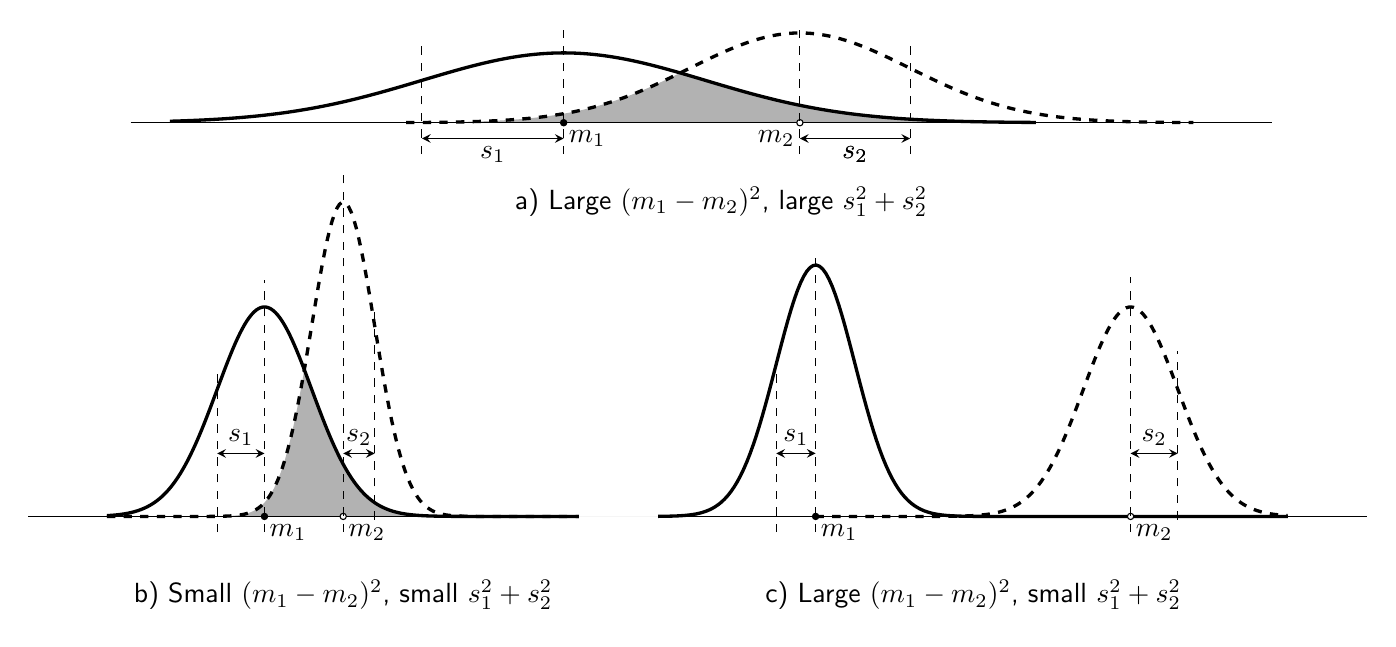
\begin{tikzpicture}[>=stealth]

% define normal distribution function 'normaltwo
\begin{scope}[scale = 2]
    \def\s{.9}
    \def\ss{.7}
    \def\m{3}
    \def\mm{4.5}
    \def\normaltwo{\x,{1/(sqrt(pi * 2*\s^2)) *exp((-(\x-\m)^2)/(2*\s^2))}}
    \def\normalone{\x,{1/(sqrt(pi * 2*\ss^2)) *exp((-(\x-\mm)^2)/(2*\ss^2))}}
    \def\ii{3.75}
    % Shade orange area underneath curve.
    \fill [fill=gray!60] (2, 0)  --  plot[domain=2:\ii, samples = 100,] (\normalone)  --  plot[domain=\ii:6, samples = 50] (\normaltwo)  --  (4,0)  --  cycle;

    % % Draw and label normal distribution function
    \draw (.25, 0)  --  (7.5,0);
    \draw[color=black,domain=.5:6, samples = 200, very thick] plot (\normaltwo) node[right] {};
    \draw[color=black, dashed, domain=2:7, samples = 200, very thick] plot (\normalone) node[right] {};

    \node  at (\m +.15, -.1) {$m_1$};
    \node  at (\mm - .15, -.1) {$m_2$};
    \node  at (\m - .5*\s, -.2) {$s_1$};
    \node  at (\mm + .5*\ss, -.2) {$s_2$};
    \draw [fill = black] (\m, 0) circle (.2mm);
    \draw [fill = white] (\mm, 0) circle (.2mm);

    % verticle lines 
    \draw [dashed, black] (\m, -.2)  --  (\m, .6);
    \draw [dashed, black] (\m-\s, -.2)  --  (\m-\s, .5);
    \draw [dashed, black] (\mm, -.2)  --  (\mm, .6);
    \draw [dashed, black] (\mm+\ss, -.2)  --  (\mm+\ss, .5);
    \draw [<->] (\m-\s, -.1)  --  (\m, -.1);
    \draw [<->] (\mm+\ss, -.1)  --  (\mm, -.1);
    
    \node  at (\mm + .5*\ss, -.2) {$s_2$};
    % subcaption
    \node [scale = 1] at (4, -.5) {a) Large $(m_1 - m_2)^2$, large $s_1^2 + s_2^2$};
\end{scope}

\begin{scope}[xshift = -3.8cm, yshift = -5cm, scale = 2]
   \def\s{.3}
    \def\ss{.2}
    \def\m{3}
    \def\mm{3.5}
    \def\normaltwo{\x,{1/(sqrt(pi * 2*\s^2)) *exp((-(\x-\m)^2)/(2*\s^2))}}
    \def\normalone{\x,{1/(sqrt(pi * 2*\ss^2)) *exp((-(\x-\mm)^2)/(2*\ss^2))}}
    \def\ii{3.25}
    % Shade orange area underneath curve.
    \fill [fill=gray!60] (2, 0)  --  plot[domain=2:\ii, samples = 100,] (\normalone)  --  plot[domain=\ii:6, samples = 50] (\normaltwo)  --  (4,0)  --  cycle;

    % % Draw and label normal distribution function
    \draw (1.5, 0)  --  (5,0);
    \draw[color=black,domain=2:5, samples = 200, very thick] plot (\normaltwo) node[right] {};
    \draw[color=black, dashed,domain=2:5, samples = 200, very thick] plot (\normalone) node[right] {};

    \node  at (\m +.15, -.1) {$m_1$};
    \node  at (\mm + .15, -.1) {$m_2$};
    \node  at (\m - .5*\s, .5) {$s_1$};
    \node  at (\mm + .5*\ss, .5) {$s_2$};
    \draw [fill = black] (\m, 0) circle (.2mm);
    \draw [fill = white] (\mm, 0) circle (.2mm);

    \draw [dashed, black] (\m, -.1)  --  (\m, 1.5);    
    \draw [dashed, black] (\m-\s, -.1)  --  (\m-\s, .95);
    \draw [dashed, black] (\mm, -.1)  --  (\mm, 2.2);
    \draw [dashed, black] (\mm+\ss, -.02)  --  (\mm+\ss, 1.35);

    \draw [<->] (\m-\s, .4)  --  (\m, .4);
    \draw [<->] (\mm+\ss, .4)  --  (\mm, .4);
    \node [scale = 1] at (3.5, -.5) {b) Small $(m_1 - m_2)^2$, small $s_1^2 + s_2^2$};
\end{scope} 

\begin{scope}[xshift = 5.2cm, yshift = -5cm, scale = 2]
   \def\s{.25}
    \def\ss{.3}
    \def\m{2}
    \def\mm{4}
    \def\normaltwo{\x,{1/(sqrt(pi * 2*\s^2)) *exp((-(\x-\m)^2)/(2*\s^2))}}
    \def\normalone{\x,{1/(sqrt(pi * 2*\ss^2)) *exp((-(\x-\mm)^2)/(2*\ss^2))}}
    % \def\ii{3.25}
    % Shade orange area underneath curve.
    % \fill [fill=gray!60] (2, 0)  --  plot[domain=2:\ii, samples = 100,] (\normalone)  --  plot[domain=\ii:6, samples = 50] (\normaltwo)  --  (4,0)  --  cycle;

    % % Draw and label normal distribution function
    \draw (1, 0)  --  (5.5,0);
    \draw[color=black,domain=1:5, samples = 200, very thick] plot (\normaltwo) node[right] {};
    \draw[color=black, dashed,domain=2:5, samples = 200, very thick] plot (\normalone) node[right] {};

    \node  at (\m +.15, -.1) {$m_1$};
    \node  at (\mm + .15, -.1) {$m_2$};
    \node  at (\m - .5*\s, .5) {$s_1$};
    \node  at (\mm + .5*\ss, .5) {$s_2$};
    \draw [fill = black] (\m, 0) circle (.2mm);
    \draw [fill = white] (\mm, 0) circle (.2mm);

    \draw [dashed, black] (\m, -.1)  --  (\m, 1.65);    
    \draw [dashed, black] (\m-\s, -.1)  --  (\m-\s, .95);
    \draw [dashed, black] (\mm, -.1)  --  (\mm, 1.52);
    \draw [dashed, black] (\mm+\ss, -.02)  --  (\mm+\ss, 1.05);

    \draw [<->] (\m-\s, .4)  --  (\m, .4);
    \draw [<->] (\mm+\ss, .4)  --  (\mm, .4);

    \node [scale = 1] at (3, -.5) {c) Large $(m_1 - m_2)^2$, small $s_1^2 + s_2^2$};
\end{scope} 


\end{tikzpicture}
\end{document}